\section{Concavity and Inflection Points}
\label{sec:concavity}

\subsection{Second Derivative and Concavity}

\begin{definition}
Graphically, a function is {\bf concave up}\index{Concave up} if its graph is curved with the opening upward (Figure \ref{fig:3-3-concavity}(a)). Similarly, a function is {\bf concave down}\index{Concave down} if its graph opens downward (Figure \ref{fig:3-3-concavity}(b)).

Concave up: looks like a cup.

Concave down: looks like a frown.


If $f''(x)$ is positive on an interval, the graph of $y=f(x)$ is concave up on that interval. We can say that $f(x)$ is increasing (or decreasing) at an increasing rate.

If $f''(x)$ is negative on an interval, the graph of $y=f(x)$ is concave down on that interval. We can say that $f(x)$ is increasing (or decreasing) at a decreasing rate.
\end{definition}

\begin{figure}[!ht]
  \centering
    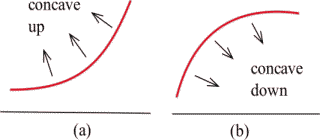
\includegraphics[width=0.4\textwidth]{img/chap3/image044.png}
    \caption{Concave up and down.}
    \label{fig:3-3-concavity}
\end{figure}
Figure \ref{fig:3-3-concavity2} shows the concavity of a function at several points. Notice that a function can be concave up regardless of whether it is increasing or decreasing.

\begin{figure}[!ht]
  \centering
    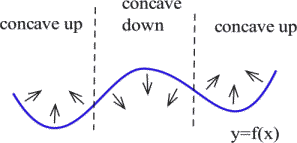
\includegraphics[width=0.4\textwidth]{img/chap3/image045.png}
    \caption{Concave up and down.}
    \label{fig:3-3-concavity2}
\end{figure}

For example, suppose an epidemic has started, and you, as a member of Congress, must decide whether the current methods are effectively fighting the spread of the disease or whether more drastic measures and more money are needed. In Figure \ref{fig:3-3-epidemic} below, $f(x)$ is the number of people who have the disease at time $x$, and two different situations are shown. In both Figure \ref{fig:3-3-epidemic}(a) and Figure \ref{fig:3-3-epidemic}(b), the number of people with the disease, $f(now)$, and the rate at which new people are getting sick, $f'(now)$, are the same. The difference in the two situations is the concavity of $f(x)$, and that difference in concavity might have a big effect on your decision.

\begin{figure}[!ht]
  \centering
    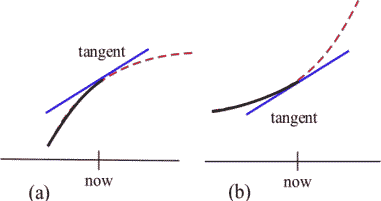
\includegraphics[width=0.4\textwidth]{img/chap3/image046.png}
    \caption{Epidemic models}
    \label{fig:3-3-epidemic}
\end{figure}
In Figure \ref{fig:3-3-epidemic}(a), $f(x)$ is concave down at ``now,'' the slopes are decreasing, and it looks as if the epidemic is tailing off. We can say ``$f(x)$ is increasing at a decreasing rate.'' It appears that the current methods are starting to bring the epidemic under control.

In Figure \ref{fig:3-3-epidemic}(b), $f(x)$ is concave up, the slopes are increasing, and it looks as if it will keep increasing faster and faster. It appears that the epidemic is still out of control.

The differences between the graphs come from whether the derivative is increasing or decreasing.

The derivative of a function $f(x)$ is a function that gives information about the slope of $y=f(x)$. The derivative tells us if the original function is increasing or decreasing.

Because $f'(x)$ is a function, we can take its derivative. This second derivative also gives us information about our original function, $f(x)$. The second derivative gives us a mathematical way to tell how the graph of a function is curved. The second derivative tells us if the original function is concave up or down.


\subsection{Inflection Points}

\begin{definition}[Inflection Point\index{Inflection point}\index{Point!inflection}]
An {\bf inflection point} of a curve is a point on the graph where the concavity of the curve changes, from concave up to down or from concave down to up.
\end{definition}

\begin{example}
Which of the labeled points in the graph in Figure \ref{fig:3-3-graph} are inflection points?

\begin{figure}[!ht]
  \centering
    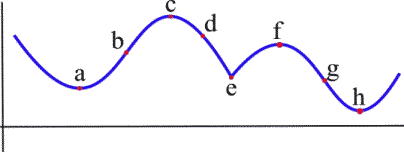
\includegraphics[width=0.4\textwidth]{img/chap3/image047.png}
    \caption{Sample curve}
    \label{fig:3-3-curve}
\end{figure}
\begin{solution} The concavity changes at points $b$ and $g$. At points $a$ and $h$, the graph is concave up on both sides, so the concavity does not change. At points $c$ and $f$, the graph is concave down on both sides. At point $e$, even though the graph looks strange there, the graph is concave down on both sides – the concavity does not change. Therefore, only points $b$ and $g$ are inflection points on the curve.
\end{solution}\end{example}

Because we know the connection between the concavity of a function and the sign of its second derivative, we can use this to find inflection points.

\begin{theorem}
If $(a, f(a))$ is an inflection point of the curve $y=f(x)$, then either $f''(a) = 0$ or $f''(a)$ is undefined. 
\end{theorem}
So to find the inflection points of a function we only need to check the points where $f''(x)$ is 0 or undefined.

Note that it is not enough for the second derivative to be zero or undefined at a point on the curve $y=f(x)$. We still need to check that $f''(x)$ changes sign at that point. The functions in the next example illustrate what can happen.

\begin{example}
Let $f(x)=x^3$, $g(x)=x^4$ and $h(x)=x^{1/3}$. For which of these functions is the point $(0,0)$ an inflection point?

\begin{figure}[!ht]
  \centering
    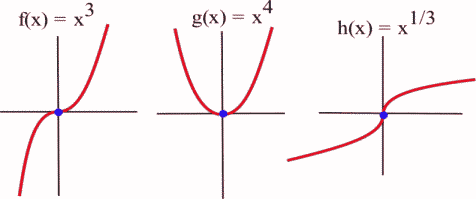
\includegraphics[width=0.4\textwidth]{img/chap3/image048.png}
    \caption{Examples and nonexamples of inflection points}
    \label{fig:3-3-curves}
\end{figure}

\begin{solution} Graphically, it is clear that the concavity of $y=f(x)=x^3$ and $y=h(x)=x^1/3$ changes at the point $(0,0)$, so $(0,0)$ is an inflection point of the curves $y=f(x)$ and $y=h(x)$. The curve $y=f(x)$ goes from concave down to concave up and the curve $y=h(x)$ goes from concave up to concave down. The function $g(x)=x^4$ is concave up everywhere (except at the point $(0,0)$), so $(0,0)$ is not an inflection point of the curve $y=g(x)$.

We can also compute the second derivatives and check the sign change.

If $f(x)=x^3$, then $f'(x)=3x^2$ and $f''(x)=6x$. The only point at which $f''(x)=0$ or is undefined ($f'(x)$ is not differentiable) is at $x=0$. If $x<0$, then $f''(x)<0$ so $y=f(x)$ is concave down. If $x>0$, then $f''(x)>0$, so $y=f(x)$ is concave up. At $x=0$, the concavity changes so the point $(0,f(0))=(0,0)$ is an inflection point of the curve $y=f(x)=x^3$.

If $g(x)=x^4$, then $g'(x)=4x^3$ and $g''(x)=12x^2$. The only point at which $g''(x)=0$ or is undefined is at $x=0$. If $x<0$, then $g''(x)>0$ so $y=g(x)$ is concave up. If $x>0$, then $g''(x)>0$, so $y=g(x)$ is also concave up. At $x=0$, the concavity does not change, so the point $(0,g(0))=(0,0)$ is not an inflection point of the curve $y=g(x)=x^4$. Keep this example in mind!

If $h(x)=x^{1/3}$, then $h'(x)=\dfrac{1}{3}x^{-2/3}$ and $h''(x)=-\dfrac{2}{9}x^{-5/3}$. $h''(x)$ is not defined at $x=0$, but if $x<0$, then $h''(x)>0$ and if $x>0$, then $h''(x)<0$, so $y=h(x)$ changes concavity at the point $(0,h(0)) = (0,0)$ and $(0,0)$ is an inflection point of the curve $y=h(x)=x^{1/3}$.
\end{solution}\end{example}

\begin{example}
\label{ex:3-3-sketches}
Sketch the graph of a function, $f(x)$ with $f(2)=3$, $f'(2)=1$, and an inflection point at the point $(2,3)$.

\begin{solution} Two possible solutions are shown in Figure \ref{fig:3-3-sketches}.

\begin{figure}[!ht]
  \centering
    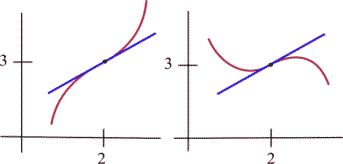
\includegraphics[width=0.4\textwidth]{img/chap3/image049.png}
    \caption{Two possible solutions to Example \ref{ex:3-3-sketches}.}
    \label{fig:3-3-sketches}
\end{figure}
\end{solution}\end{example}
